\documentclass[11pt,a4paper,final]{article}
\usepackage[utf8x]{inputenc}
\usepackage{ucs}
\usepackage{amsmath}
\usepackage{amsfonts}
\usepackage{float}
\usepackage{amssymb}
\usepackage[final]{graphicx}
\usepackage{setspace}
\usepackage[final]{listings}
\usepackage[final]{pdfpages}
\usepackage{color}
\usepackage{bm}
\usepackage{microtype}
\onehalfspacing
\author{Marc Ferriggi}
\title{Machine Learning 1 Worksheet Report}

\definecolor{codegreen}{rgb}{0,0.6,0}

\lstdefinestyle{mystyleR}{  
	commentstyle=\color{codegreen},
	breakatwhitespace=false,         
	breaklines=true,                 
	captionpos=b,                    
	keepspaces=true,                 
	numbers=left,                    
	numbersep=5pt,                  
	showspaces=false,                
	showstringspaces=false,
	showtabs=false,                  
	tabsize=2
}

\begin{document}
	\title{Machine Learning 1 \\
	\large ICS2207 \\ Assignment Report}
	\author{Marc Ferriggi (286397M)}
	\date{\today}
	\maketitle
	\tableofcontents
	%\listoffigures
	%\listoftables
	%\lstlistoflistings
	
	\pagebreak
	\section{Introduction}
	\label{Intro}
	\paragraph{} The Travelling Salesman Problem is a very common problem in the field of operations research. This has been studied extensively by mathematicians, computer scientists, and many great minds yet its complexity is still unknown \cite{TSP}. The problem statement is given as follows:\\
	\hspace{0pt}\\
	``Given a collection of cities and the cost of travel between each pair of them, the travelling salesman problem, or TSP for short, is to find the cheapest way of visiting all of the cities and returning to your starting point." \cite{TSP}\\
	\par Traditional methods for solving this problem come in three types; calculus based methods, exhaustive search methods and random search methods \cite{Goldberg}. These methods, however, pose a large number of problems such as the algorithm converging to a local optimum or running in exponential time. Machine Learning Algorithms such as Genetic Algorithms (GAs) or the Ant-Colony Optimisation method (ACO) can be used to find accurate approximations to the solutions to the TSP and other similar optimisation problems. \\
	\par In order to solve this problem using a Genetic Algorithm (Section \ref{GAs}) and the ACO method (Section \ref{ACO}), a few assumptions were made. Firstly, it was assumed that the data provided will come from a symmetric instance of TSP, i.e. the distance $d$ from city $c_i$ to city $c_j$ $d(c_i,c_j)=d(c_j,c_i)$ $\forall i,j\in [1,n]$. Another assumption that's being made is that the ``closed" version of TSP will be solved for this task, i.e. the salesman will end in the city where he started.\\
	\par In Section \ref{GAs} of this paper, Genetic Algorithms shall be defined and a method to solve the TSP using such an algorithm will be proposed. Section \ref{ACO} shall define Ant-Colony Optimisation and propose a method for solving the TSP using this method. Section \ref{Results} will then compare the outcomes of the two algorithms and these results shall be discussed in detail. All code used will be listed in the Appendix (Section \ref{Appendix}). 
	\section{Genetic Algorithms}
	\label{GAs}
	\paragraph{} Genetic algorithms are designed to simulate a biological process \cite{GeneticAlgorithms}, thus most of the terminology refers to the algorithm's biological counterpart. The components that make up GAs are as follows:
	\begin{itemize}
		\item an objective (or fitness) function
		\item a population of chromosomes
		\item a selection operator on the chromosomes
		\item a crossover function which produces a new generation of chromosomes
		\item a random mutation function
	\end{itemize}
	\par The objective function is the function that the algorithm is trying to optimise. In Genetic Algorithms, this is often referred to as a \textit{fitness} function, this term is in fact taken from evolutionary theory \cite{GeneticAlgorithms}. For the TSP, the fitness function is the sum of the distances between the points, the TSP in fact deals with minimising this sum in order to be able to find the shortest path. Given that the data under study is given in coordinate format \cite{data}, the fitness function used for the TSP is given in Equation \ref{fitness} \cite{GeneticAlgorithms}.
	\begin{equation}
	\label{fitness}
	D=\sum_{k=1}^{n}\sqrt{(x_{k+1}-x_k)^2+(y_{k+1}-y_k)^2}
	\end{equation}
	\par A chromosome refers to a value that will be considered as the candidate solution to the optimisation problem. In the case of the TSP, the chromosome could be a permutation of the cities which represent the order that the salesman visits each city. Historically, chromosomes were encoded as a bit string, however it would make more sense not to encode it in this way for the TSP, this however will require a change in the crossover and mutation functions \cite{GeneticAlgorithms}.\\
	\par The selection operator refers to the method used to select which chromosomes are to be chosen for reproduction. In general, a fitter chromosome should be more likely to be selected. In the case of TSP, the probability function must be changed slightly from the original definition since the objective of the TSP is to minimize the fitness function (cost) and not maximize it, thus care must be taken to reverse the probability function. \\
	\par Once the ``fittest" chromosomes are selected, the crossover operator is then used to ``combine" them. This operator ``resembles the biological crossing over and recombination of chromosomes to create two offspring" \cite{GeneticAlgorithms}. In the case of the TSP, special care needs to be taken when designing this function and the classical way of defining this operator will not work since each city needs to be visited only once \cite{Haupt}. The technique which shall be used in the implementation for the TSP is known as the ``cycle" crossover (as taken from \cite{GeneticAlgorithms}) and works as follows:
	\begin{enumerate}
		\item Initially, a random location is chosen in the length of the chromosome.
		\item The two parent chromosomes exchange integers at this point to create the offspring.
		\item If the integers are the same value then the offspring is the same as the parent and the algorithm terminates.
		\item Otherwise, each offspring now has a duplicate integer, so switch the duplicate integer in the first offspring with the integer in the same location in the second offspring.
		\item Repeat the above step until there are no duplicates in the first offspring (and thus the second offspring).
		\item Both are now valid permutations.
	\end{enumerate}
	\par The importance of the mutation step is to reduce the probability of the algorithm converging to a local optimum \cite{Haupt}. This is achieved by causing the algorithm to maintain diversity in the population, however it can cause it to converge more slowly \cite{GeneticAlgorithms}. Again, since the chromosome for the TSP is not encoded as a bit string, the mutation operator changes slightly from that described by Haupt in the original definition of a Genetic Algorithm. The implemented mutation operator randomly chooses two integers in a chromosome from the new generation and swaps them \cite{GeneticAlgorithms}. This will happen with a rather low probability in order to increase the rate of convergence.
	
	\section{Ant-Colony Optimisation}
	\label{ACO}
	\paragraph{} The Ant-colony Optimisation algorithm forms part of a class of population-based algorithms known as swarm intelligence (SI) that considers the collective behaviour of the population and individual solutions \cite{fastACO}. A general ACO algorithm has the following form \cite{scholarACO}:\\
	\begin{lstlisting}
	Set parameters, initialize pheromone trails
	SCHEDULE ACTIVITIES
		ConstructAntSolutions
		DaemonActions  {optional}
		UpdatePheromones
	END_SCHEDULE_ACTIVITIES
	\end{lstlisting}
	
	\par The parameters initialised for my implementation of the Ant Colony Optimisation Algorithm are as follows:
	\begin{enumerate}
		\item \underline{no\_of\_ants}: the number of ants in each iteration.
		\item \underline{max\_iter}: the maximum number of iterations.
		\item \underline{evaporation\_rate}: the rate at which the pheromones evaporate.
		\item \underline{alpha}: a parameter for calculating the probability of an ant selecting a certain route. Alpha gives more weighting to the pheromone values.
		\item \underline{beta}: a parameter for calculating the probability of an ant selecting a certain route. Beta gives more weighting to the heuristic value.
		\item \underline{q0}: this parameter gives the probability of using the previous ants' experience over selecting a random path.
	\end{enumerate} 
	\par Since the task at hand is to write an algorithm to solve the symmetric TSP and R is optimised for working with matrix algebra, the distances between each city were calculated as an initialisation step in order to avoid having to compute these values each time on every ant run. The distances between each city were stored in a symmetric matrix thus only the lower triangular matrix needed to be worked out using for loops.\\
	
	\par In order to construct the ant solutions, initially, each ant is placed at random on a city. At each step, the ant then chooses the next city based on the probability matrix given in Equation \ref{ACOProb}.
	
	\begin{equation}
	\label{ACOProb}
	p^k_{ij}(t)=\frac{[\tau_{ij}(t)]^{\alpha}.[\eta_{ij}]^{\beta}}{\sum_{l\in\mathcal{N}^k_i}[\tau_{il}(t)]^{\alpha}.[\eta_{il}]^{\beta}}\ if\ j\in\mathcal{N}^k_i
	\end{equation}
	Where $p^k_{ij}(t)$ is the probability that ant $k$ goes to city $j$ from city $i$ at iteration $t$, $\tau_{ij}(t)$ is the pheromone value on edge $ij$ at iteration $t$, $\eta_{ij}$ is the heuristic value on edge $ij$ and $\mathcal{N}^k_i$ is the set of all possible nodes reachable by ant $k$ from node $i$ which in our case will be the set of all possible nodes not yet visited by ant $k$ \cite{GargACO}.\\
	
	\par The ant with the best solution after each iteration will then update the pheromone values of each edge and is defined as seen in Equation \ref{pheromoneUpdate} \cite{fastACO}.
	\begin{equation}
	\label{pheromoneUpdate}
	\begin{split}
	\tau_{ij} &= (1-\rho)\tau_{ij}+\rho\sum_{k=1}^{m}\triangle\tau_{ij}^{k},\\
	\triangle\tau_{ij}^{k} &=\frac{1}{L^k}
	\end{split}	
	\end{equation}
	Where $m$ is the number of ants, and $L^k$ is the length of the best tour of that iteration. All pheromone values also evaporate at a rate defined by the parameter after each iteration.
	\section{Results and Comparisons}
	\label{Results}
	\paragraph{ }In general, when comparing the performance of the ACO Algorithm to the GA algorithm, one can note that the ACO algorithm seems to find a better approximation to the solution than the GA, and it does it in much less time using less iterations. This section compares the results of both algorithms on specific instances. By simply looking at the plots of the standard error of our estimated value compared with the iteration number, one can note the significant difference in performance. Note that with very large numbers, the Genetic Algorithm would take a very long time to compute and thus all the points were normalised between 0 and 1 in order to improve the speed of the algorithm. This step was then also repeated in the ACO Algorithm in order to be able to accurately compare the 2 methods.\\
	\hspace{0pt}\\
	\textbf{Instance name: bays29.tsp}\\
	\underline{GA method:} \textit{see listing \ref{GACode}}\\
	\underline{ACO method:} \textit{see listing \ref{ACOCode}}\\
	\hspace{0pt}\\
	\begin{minipage}{0.475\textwidth}
		\textbf{\underline{GA Performance:}}\\
		\underline{Time Taken:} 177127.73ms\\
		\underline{Best Distance Found:}{\hspace{2pt}}6.129391
		\underline{Actual Optimal Distance:} 4.581227\\
		\underline{Standard Error:} 2.965736
	\end{minipage}
	\begin{minipage}{0.475\textwidth}
		\textbf{\underline{ACO Performance:}}\\
		\underline{Time Taken:} 7170.33ms\\
		\underline{Best Distance Found:}{\hspace{2pt}}4.601584
		\underline{Actual Optimal Distance:} 4.581227\\
		\underline{Standard Error:} 0.000414
	\end{minipage}	
	
	\begin{figure}[H]
		%\centering
		\begin{minipage}{.5\textwidth}
			\centering
			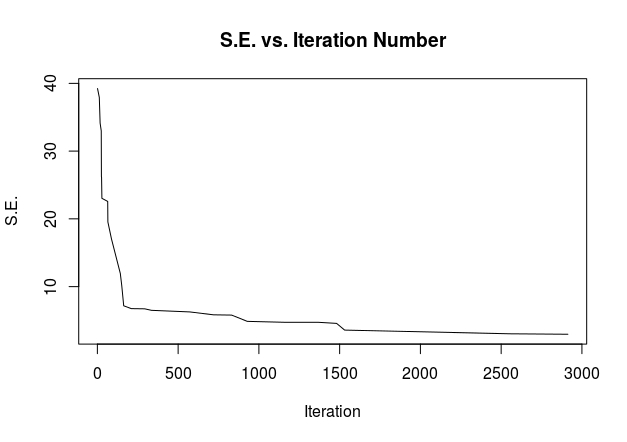
\includegraphics[scale= 0.4]{Bays29GAPlot}
			\caption{Genetic Algorithm}
			\label{fig:bays29GA}
		\end{minipage}
		\begin{minipage}{.5\textwidth}
			\centering
			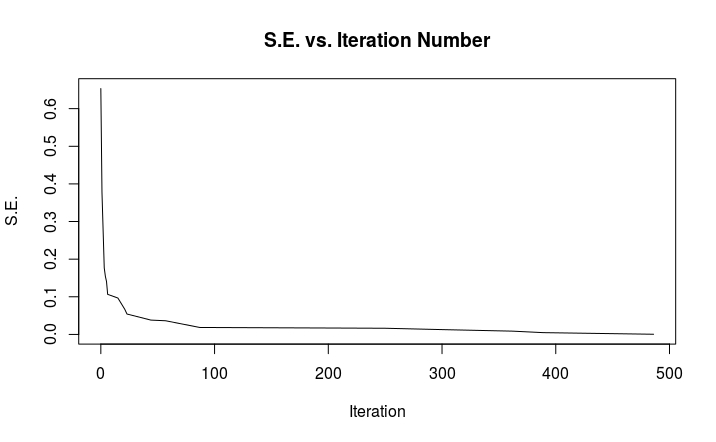
\includegraphics[scale=0.4]{Bays29ACOPlot}
			\caption{ACO Algorithm}					
			\label{fig:bays29ACO}
		\end{minipage}
	\end{figure}
	\hspace{0pt}\\
	\textbf{Instance name: att48.tsp}\\
	\underline{GA method:} \textit{see listing \ref{GACode}}\\
	\underline{ACO method:} \textit{see listing \ref{ACOCode}}\\
	\hspace{0pt}\\
	\begin{minipage}{0.475\textwidth}
		\textbf{\underline{GA Performance:}}\\
		\underline{Time Taken:} 475314.39ms\\
		\underline{Best Distance Found:}{\hspace{2pt}}8.432387
		\underline{Actual Optimal Distance:} 5.377854\\
		\underline{Standard Error:} 9.330172
	\end{minipage}
	\begin{minipage}{0.475\textwidth}
		\textbf{\underline{ACO Performance:}}\\
		\underline{Time Taken:} 49082.17ms\\
		\underline{Best Distance Found:}{\hspace{2pt}}5.431998
		\underline{Actual Optimal Distance:} 5.377854\\
		\underline{Standard Error:} 0.00101
	\end{minipage}
	
	\begin{figure}[H]
		%\centering
		\begin{minipage}{.5\textwidth}
			\centering
			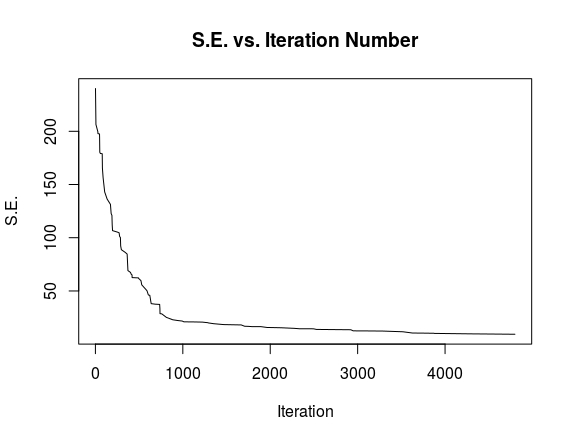
\includegraphics[scale= 0.4]{att48GAGraph}
			\caption{Genetic Algorithm}
			\label{fig:att48GA}
		\end{minipage}
		\begin{minipage}{.5\textwidth}
			\centering
			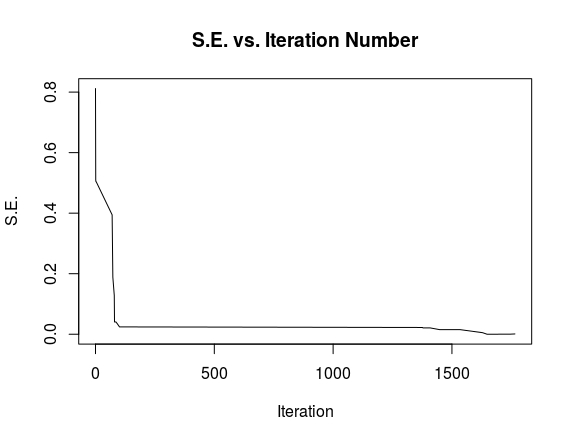
\includegraphics[scale=0.4]{Att48ACO}
			\caption{ACO Algorithm}					
			\label{fig:att48ACO}
		\end{minipage}
	\end{figure}
	\hspace{0pt}\\
	\textbf{Instance name: ch130.tsp}\\
	\underline{GA method:} \textit{see listing \ref{GACode}}\\
	\underline{ACO method:} \textit{see listing \ref{ACOCode}}\\
	\hspace{0pt}\\
	\begin{minipage}{0.475\textwidth}
		\textbf{\underline{GA Performance:}}\\
		\underline{Time Taken:} 1292756.23ms\\
		\underline{Best Distance Found:}{\hspace{2pt}}26.76519
		\underline{Actual Optimal Distance:} 8.703517\\
		\underline{Standard Error:} 326.2241
	\end{minipage}
	\begin{minipage}{0.475\textwidth}
		\textbf{\underline{ACO Performance:}}\\
		\underline{Time Taken:} 57314.04ms\\
		\underline{Best Distance Found:}{\hspace{2pt}}9.542707
		\underline{Actual Optimal Distance:} 8.703517\\
		\underline{Standard Error:} 0.5555441
	\end{minipage}
	
	\begin{figure}[H]
		%\centering
		\begin{minipage}{.5\textwidth}
			\centering
			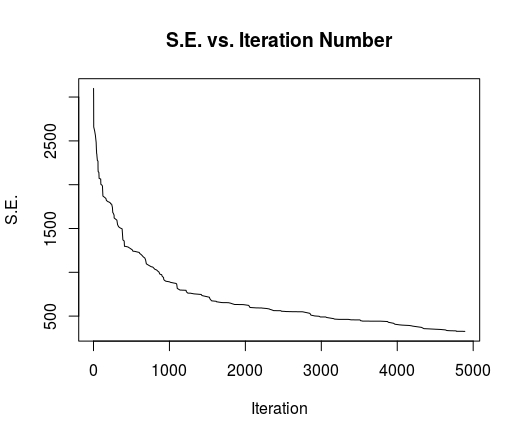
\includegraphics[scale= 0.4]{ch130GAPlot}
			\caption{Genetic Algorithm}
			\label{fig:ch130GA}
		\end{minipage}
		\begin{minipage}{.5\textwidth}
			\centering
			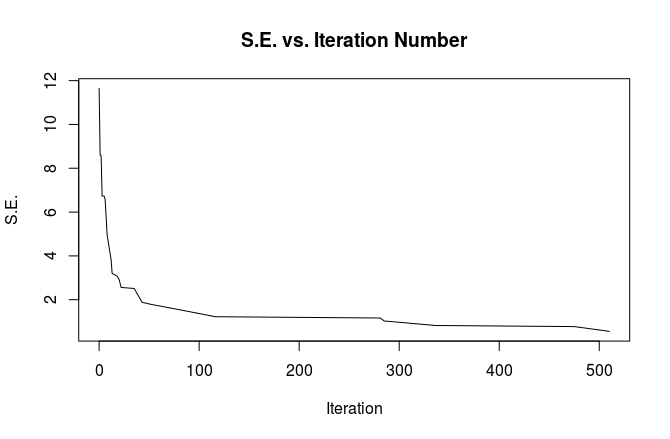
\includegraphics[scale=0.4]{ch130ACOPlot}
			\caption{ACO Algorithm}					
			\label{fig:ch130ACO}
		\end{minipage}
	\end{figure}
	\hspace{0pt}\\
	\textbf{Instance name: eli101.tsp}\\
	\underline{GA method:} \textit{see listing \ref{GACode}}\\
	\underline{ACO method:} \textit{see listing \ref{ACOCode}}\\
	\hspace{0pt}\\
	\begin{minipage}{0.475\textwidth}
		\textbf{\underline{GA Performance:}}\\
		\underline{Time Taken:} 893826.54ms\\
		\underline{Best Distance Found:}{\hspace{2pt}}19.80362
		\underline{Actual Optimal Distance:} 8.863002\\
		\underline{Standard Error:} 119.6971
	\end{minipage}
	\begin{minipage}{0.475\textwidth}
		\textbf{\underline{ACO Performance:}}\\
		\underline{Time Taken:} 30574.32ms\\
		\underline{Best Distance Found:}{\hspace{2pt}}9.75988
		\underline{Actual Optimal Distance:} 8.863002\\
		\underline{Standard Error:} 0.6458297
	\end{minipage}
	
	\begin{figure}[H]
		%\centering
		\begin{minipage}{.5\textwidth}
			\centering
			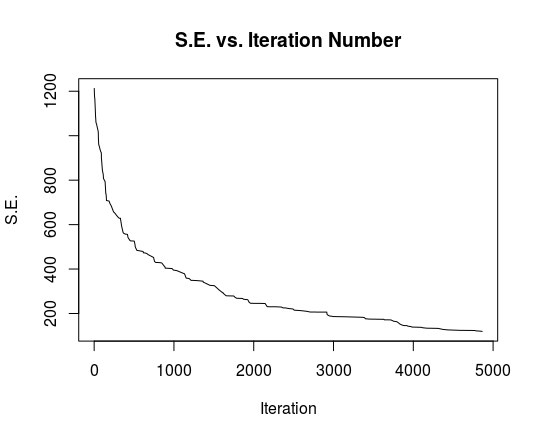
\includegraphics[scale= 0.4]{eli101GAPlot}
			\caption{Genetic Algorithm}
			\label{fig:eli101GA}
		\end{minipage}
		\begin{minipage}{.5\textwidth}
			\centering
			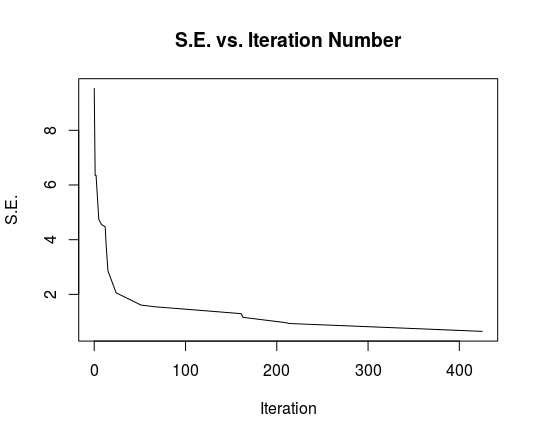
\includegraphics[scale=0.4]{eli101ACOPlot}
			\caption{ACO Algorithm}					
			\label{fig:eli101ACO}
		\end{minipage}
	\end{figure}		
	\subsection{Methods for Improving the Performance of the Algorithms}
	\paragraph{ }As can be clearly seen from the results above, the performance of the Genetic Algorithm is not great when compared to that of the ACO Algorithm. Here are some methods to possibly improve the performance of this algorithm.
	\begin{enumerate}
		\item The first obvious thing to do would be to adjust the parameters for each example until a combination is found which would provide a better solution.
		\item When looking at Figure \ref{fig:ch130GA} it can be noted that the algorithm was still finding better solutions at higher iterations, increasing the maximum number of iterations for examples with  larger number of cities would also help improve the algorithm's performance.
		\item Another optimisation step would be to change the selection operator of the GA. In its current state its possible for the algorithm to always select the same chromosomes as that solution improves since the probability value of a particular chromosome could approach 1. Possible workarounds to this would be to use a rank-based method \cite{rank} or a tournament based method \cite{tournament}.
	\end{enumerate}
	
	\section{Conclusion}
	\label{Conc}
	\paragraph{ }In this paper we have seen two methods to approximate the solution to the symmetric Travelling Salesman Problem using Machine Learning Algorithms written in R. The written Ant Colony Optimisation algorithm seems to be clearly superior to the Genetic Algorithm in both speed and accuracy and from our plots it would seem that it also converges at a much faster rate. We also have seen methods of possibly improving the Genetic Algorithm's performance. Using Machine Learning algorithms to find reasonable solutions to NP Hard problems can be used as a very powerful tool in computer science and can give accurate results when done right. 
	
	\section{Statement of Completion}
	\label{SoC}
	\begin{table}[H]
		\centering
		\begin{tabular}{|l|c|}
			\hline
			\textbf{Item} & \textbf{Completed(Yes/No/Partial)}\\
			\hline
			\hline
			Implemented GA & Yes\\\hline
			Implemented ACO & Yes\\\hline
			Evaluated GA vs ACO for selected instances & Yes\\\hline
			Described GA architecture in report & Yes\\\hline
			Described ACO architecture in report & Yes\\\hline
		\end{tabular}
	\end{table}
	\pagebreak
	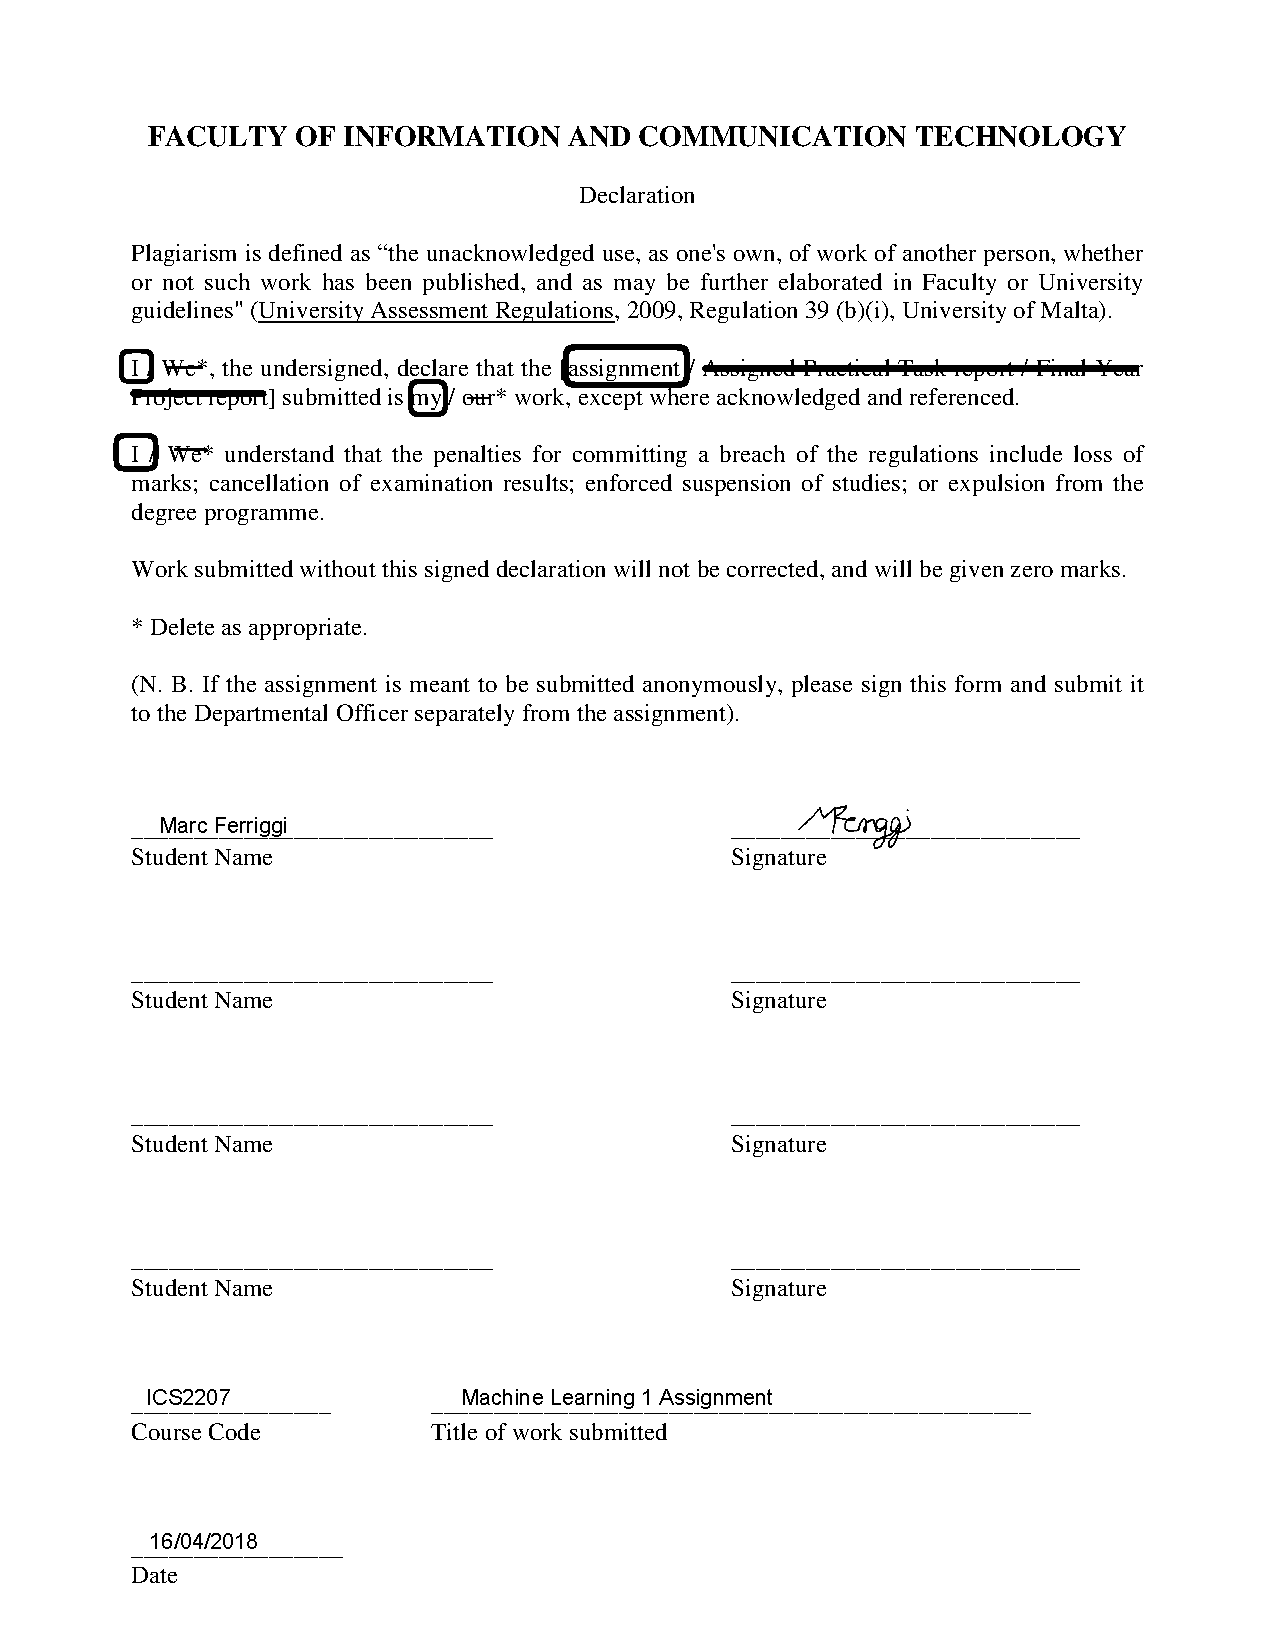
\includepdf[pages=1,pagecommand={\section{Plagiarism Declaration Form} \thispagestyle{empty}}, scale=0.75]{PDF.pdf}
	%\section{}
	%\label{PlagForm}
	%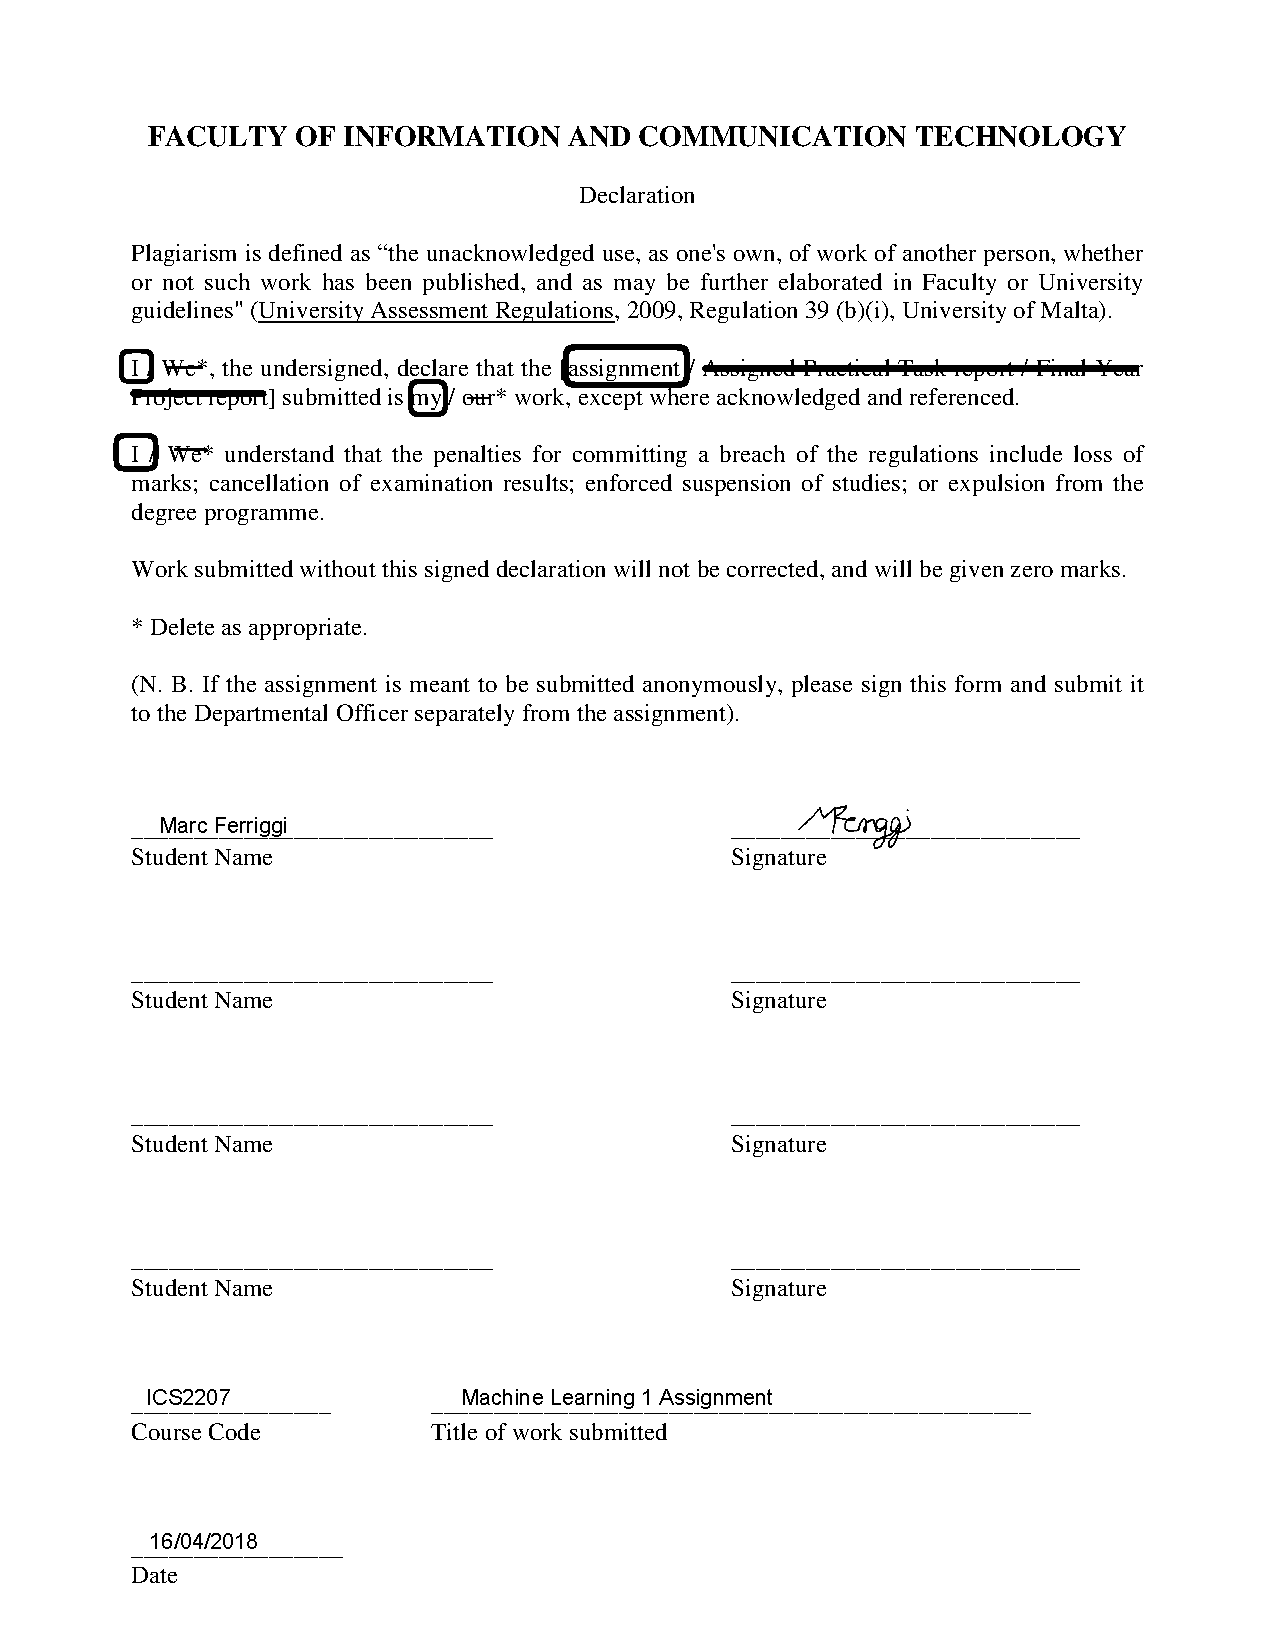
\includepdf[scale=0.6]{PDF.pdf}
	\section{Appendix}
	\label{Appendix}
	%Code Listings
	\lstset{style=mystyleR}
	\begin{lstlisting}[language = R,caption= Genetic Algorithm Code,label=GACode]
	rm(list=ls()) #Clear Environment
	
	require(readxl) #needed to import data
	Data = read_xlsx(file.choose(),col_names=FALSE) #Choose the data file you want to open
	X = Data[2] #X coordinates indexed by city
	Y = Data[3] #Y coordinats indexed by city
	rm(Data) #remove Data (not needed)
	
	#Normalize points to be between 0 and 1
	#This is an optimisation step to improve the speed of the function
	X = X/max(X)
	Y = Y/max(Y)
	
	#fitnessFunction:
	#takes a population of chromosomes in Matrix form as an argument
	#returns a vector of distances each element corresponding to a chromosome
	#Example of use:
	#a = c(1,2,3,4,5,6,7)
	#b = c(2,4,3,1,5,15,12)
	#c = c(10,2,3,1,5,6,11)
	#pop = t(cbind(a,b,c))
	#distances=fitnessFuntion(pop)
	fitnessFunction <- function(pop) {
		Npop = nrow(pop)#size of population
		Ncity = ncol(pop)#no. of cities
		#append first city to the end in order to be able to calculate the distance
		tour = cbind(pop,pop[,1]) 
		#Empty vector to store distances of each chromosome
		distances = mat.or.vec(Npop,1)
	
		#loop over every tour in the population
		for (i in 1:Npop) {
			chromosome = tour[i,]
			#for every city in the chromosome
			distance = 0
			for (j in 1:Ncity){
				#fitness function as defined in Equation 1 of my Documentation
				temp = 		sqrt(((X[chromosome[j+1],1]-X[chromosome[j],1])^2+(Y[chromosome[j+1],1]-Y[chromosome[j],1])^2))
				distance = distance + temp
			}
			distances[i]=distance
		}
		distances
	}
	
	#mate function, mates 2 chromosomes given a pointer as
	#the starting pointer and returns a list of the 2 new 
	#child chromosomes
	mate <- function(mate1,mate2,pointer) {
		temp = mate1
		change = TRUE
		#loop until all values are unique
		while (change) {
			#swap values
			mate1[pointer]=mate2[pointer]
			mate2[pointer]=temp[pointer]
			#returns an array of indices which match the value at mate1[pointer]:
			pointers = which(mate1==mate1[pointer],arr.ind = TRUE) 
			#check if there exists an duplicate in the chromosome
			change = FALSE
			tempPointer = pointer
			for (j in 1:length(pointers)) {
				if (pointers[j]!=pointer) {
					#if there's a duplicate, point to it
					tempPointer = pointers[j]
					change = TRUE
				}
			}
			pointer = tempPointer
		}
		return(unname(rbind(mate1,mate2)))
	}
	
	#function that mutates the chromosome
	mutate <- function(chromosome) {
		indices = sample(1:length(chromosome),2,replace=FALSE) #choose 2 random indices in the chromosome
		#swap the elements
		swapTemp = chromosome[indices[1]]
		chromosome[indices[1]] = chromosome[indices[2]]
		chromosome[indices[2]] = swapTemp
		return(chromosome)
	}
	
	
	#Main Function:
	#Initialize Genetic Algorithm Parametes:
	NoOfCities = nrow(X) #Number of Cities
	popSize = 10 #no of chromosomes in each population
	pop = mat.or.vec(popSize,NoOfCities)
	pop2 = mat.or.vec(popSize,NoOfCities)
	best = mat.or.vec(1,NoOfCities) #vector to keep the best chromosome so far
	keep = 6 #no of chromosomes to be chosen as parents
	mutationRate = 0.4 #probability of mutation
	#noMutations = ceiling((popSize-1)*mutationRate) #total number of mutations
	Matings = ceiling((popSize-keep)/2) #number of matings
	maxit = 5000 #maximum number of iterations
	
	#optTour = c(1,28,6,12,9,5,26,29,3,2,20,10,4,15,18,17,14,22,11,19,25,7,23,27,8,24,16,13,21)#bays29
	#optTour = c(1,8,38,31,44,18,7,28,6,37,19,27,17,43,30,36,46,33,20,47,21,32,39,48,5,42,24,10,45,35,4,26,2,29,34,41,16,22,3,23,14,25,13,11,12,15,40,9)#att48
	optTour = c(1,41,39,117,112,115,28,62,105,128,16,45,5,11,76,109,61,129,124,64,69,86,88,26,7,97,70,107,127,104,43,34,17,31,27,19,100,15,29,24,116,95,
			79,87,12,81,103,77,94,89,110,98,68,63,48,25,113,32,36,84,119,111,123,101,82,57,9,56,65,52,75,74,99,73,92,38,106,53,120,58,49,72,91,6,102,
			10,14,67,13,96,122,55,60,51,42,44,93,37,22,47,40,23,33,21,126,121,78,66,85,125,90,59,30,83,3,114,108,8,18,46,80,118,20,4,35,54,2,50,130,71)#ch130
	optDistance = 0
	for (i in 2:NoOfCities) {
		optDistance = optDistance + sqrt((X[optTour[i-1],1]-X[optTour[i],1])^2+(Y[optTour[i-1],1]-Y[optTour[i],1])^2)
	}
	
	bestVal = 1e+22 #Arbitrary large number
	se = (bestVal-optDistance)^2
	iteration = 0
	
	#chromosomes that will survive and mate:
	kept = mat.or.vec(keep,NoOfCities)
	#stores the probability of each chromosome to survive
	prob = mat.or.vec(popSize,1)
	
	#populate initial population with random chromosomes:
	for (i in 1:popSize) {
		pop[i,] = sample(1:NoOfCities,NoOfCities) #creates a chromosome
	}
	
	#set starting time:
	start_time = as.numeric(Sys.time())*1000;
	#MAIN LOOP:
	for (gen in 1:maxit) {
		#compute the fitness function on the population
		Lengths = fitnessFunction(pop)
		#Save the best solution 
		if (min(Lengths)<bestVal) {
			best[1,] = pop[which.min(Lengths),]
			bestVal = min(Lengths)
			se = c(se,(bestVal-optDistance)^2) #standard error for graph
			iteration = c(iteration,gen)  #iter number for graph
			end_time=as.numeric(Sys.time())*1000
			print(bestVal)
		}
	
		#selection
		total = sum(Lengths)
		#Probability of each chromosome to be selected
		for (i in 1:popSize) {
			prob[i] = 1- (Lengths[i]/total)
			#This gives a higher probability value to the shortest lengths
			#Thus we need to select the chromosomes with the highest probability
		}
		#selects the elements of the population to be kept based on the probability distribution
		#as defined above
		odds = sample(1:popSize,keep,replace=TRUE,prob = prob)
		#choose the chromosomes to be kept and store them in the new population 
		#keep the best and second best solutions
		pop2[1,]=pop[which.min(Lengths),]
		pop2[2,]=pop[which(Lengths==sort(Lengths,decreasing=TRUE)[popSize-1])[1],]
		#choose parents, we'll choose 3 mums and 3 dads, to have 6 kids:
		for (i in 1:keep) {
			#keep a record of the parents kept:
			kept[i,] = pop[odds[i],]
		}
	
		index = 3
		while (index < 9) {
			#mate1, mate2 are random integers between 1 and keep (index)
			mate1=ceiling(runif(1, min=0, max=keep-1))
			mate2=ceiling(runif(1, min=0, max=keep-1))
			pointer = ceiling(runif(1,0,NoOfCities)) #random int between 1 and NoOfCities
			children = mate(kept[mate1,],kept[mate2,],pointer) #call the mate function
			#mutate with probability and save to population
			if (runif(1)<=mutationRate) {
				pop2[index,] = mutate(children[1,])
			} else {
				pop2[index,] = children[1,]
			}
			if (runif(1)<=mutationRate) {
				pop2[index+1,] = mutate(children[2,])
			} else {
				pop2[index+1,] = children[2,]
			}
			index=index+2
		}
		#Randomly fill remaining part of population with chromosomes
		for (i in 9:10) {
			pop2[i,] = sample(1:NoOfCities,NoOfCities) #creates a chromosome
		}
	
		#Print iteration number
		if (gen%%100==0) {
			print(gen)
		}
		pop = pop2
	}
	#compute the fitness function on the population
	Lengths = fitnessFunction(pop)
	#Save the best solution 
	if (min(Lengths)<bestVal) {
		best[1,] = pop[which.min(Lengths),]
		bestVal = min(Lengths)
		se = c(se,(bestVal-optDistance)^2) #standard error for graph
		iteration = c(iteration,gen)  #iter number for graph
		end_time=as.numeric(Sys.time())*1000
		print(bestVal)
	}
	paste("Time Taken: ",end_time-start_time)
	print(best[1,])
	plot(iteration[-1],se[-1],type="l",main="S.E. vs. Iteration Number",xlab="Iteration",ylab="S.E.")
	\end{lstlisting}
	
	\begin{lstlisting}[language = R, caption= ACO Code, label=ACOCode]
	rm(list=ls()) #Clear Environment
	
	require(readxl) #needed to import data
	Data = read_xlsx(file.choose(),col_names=FALSE) #Choose the data file you want to open
	X = Data[2] #X coordinates indexed by city
	Y = Data[3] #Y coordinats indexed by city
	rm(Data) #remove Data (not needed)
	
	#Normalize points to be between 0 and 1
	#This is an optimisation step to improve the speed of the function
	X = X/max(X)
	Y = Y/max(Y)
	
	############
	#Parameters# <- adjusting these would change the performance of the algorithm
	############
	no_of_ants = 10 #no of ants in each iteration
	max_iter = 3000 #maximum number of iterations
	evaporation_rate = 0.15 #evaporation rate of pheromones
	alpha = 1 #alpha and beta are paramenters for calculating the prob matrix
	beta = 4
	q0 = 0.6 #probability of using other ant's experience
	
	###########
	#Functions#
	###########
	#this function returns the reciprocal of a number, unless that number is 0
	probValues <- function(number) {
		if (number == 0) {
			number
		} else {
			1/number
		}
	}
	
	#function that accepts a matrix with the first column being the starting point of each ant and the other columns all being 0
	#a Heuristic Matrix and the pheromone value Matrix Tau and returns tours of each ant.
	setRoutes <- function(Routes, Heuristic, Tau) {
		#for every ant:
		for (i in (1:nrow(Routes))) {
			Memory = mat.or.vec(ncol(Routes),1) #Set Ant's memory to 0s 
			Score = (Tau^alpha)*(Heuristic)^beta #Calculate score matrix
			Memory[1] = Routes[i,1] #Add starting node to memory 
			#Loop until all cities have been visited:
			for (j in 2:ncol(Routes)) {
				currentCity = Memory[j-1]
				#set score to 0 for current city:
				Score[,currentCity] = 0
				ParticularScore = Score[currentCity,]
				if (runif(1)<=q0) {
					#find the city with the largest score:
					Memory[j] = which.max(ParticularScore)
				} else {
					#Choose the next node based on probability
					Probability = ParticularScore/sum(ParticularScore)
					Memory[j] = sample(1:length(Probability),1,prob=Probability)
				}
			}
			Routes[i,] = Memory
		}
		Routes
	}
	
	#function that calculates the length of each tour
	fitnessFunction <- function(Routes, Distances) {
		sum = mat.or.vec(nrow(Routes),1)
		#for each ant j
		for (j in 1:nrow(Routes)) { 
			cities = Routes[j,]
			#for each city visited
			for (i in 1:(ncol(Routes)-1)) {
				#add up the distances
				sum[j] = sum[j] + Distances[cities[i],cities[i+1]]
			}
			sum[j] = sum[j] + Distances[cities[i+1],cities[1]]
		}
	sum
	}
	
	#function that updates pheromones after an iteration
	updatePheromones <- function(path, length, evaporation_rate, Tau) {
		for (i in 1:(length(path)-1)) {
			Tau[path[i],path[i+1]] = (1-evaporation_rate)*Tau[path[i],path[i+1]]+evaporation_rate*(length)^(-1);
			Tau[path[i+1],path[i]] = Tau[path[i],path[i+1]] 
		}
		Tau
	}
	
	#################
	#Other Variables#
	#################
	start_time=as.numeric(Sys.time())*1000;
	no_of_cities = nrow(X)
	Tau = matrix(0.00001,nrow = no_of_cities, ncol = no_of_cities) #initial pheromone matrix
	starting_nodes = mat.or.vec(no_of_ants,1)
	dontStop = TRUE
	#generate distance between cities matrix
	Distances = matrix(0,nrow = no_of_cities,ncol = no_of_cities)
	Heuristic = Distances
	iter = 0
	#Note that Distances is a symmetric matrix since we're working out the Symetric TSP
	#, thus in order to improve complexity first the lower triangular part is worked out, 
	#then its transpose is added to itself.
	for (i in 2:no_of_cities) {
		for (j in 1:i) {
			Distances[i,j] = sqrt((X[i,1]-X[j,1])^2+(Y[i,1]-Y[j,1])^2)
		}
	}
	Heuristic = apply(Distances,c(1,2),probValues) #Genarate the Heuristic Matrix (see function probValues)
	Distances = Distances + t(Distances)
	Heuristic = Heuristic + t(Heuristic)
	
	bestRoute = mat.or.vec(no_of_cities,1)
	bestLength = 1e27 #Arbitrarily large number
	
	#optTour = c(1,28,6,12,9,5,26,29,3,2,20,10,4,15,18,17,14,22,11,19,25,7,23,27,8,24,16,13,21)#bays29
	#optTour = c(1,8,38,31,44,18,7,28,6,37,19,27,17,43,30,36,46,33,20,47,21,32,39,48,5,42,24,10,45,35,4,26,2,29,34,41,16,22,3,23,14,25,13,11,12,15,40,9)#att48
	optTour = c(1,41,39,117,112,115,28,62,105,128,16,45,5,11,76,109,61,129,124,64,69,86,88,26,7,97,70,107,127,104,43,34,17,31,27,19,100,15,29,24,116,95,
				79,87,12,81,103,77,94,89,110,98,68,63,48,25,113,32,36,84,119,111,123,101,82,57,9,56,65,52,75,74,99,73,92,38,106,53,120,58,49,72,91,6,102,
				10,14,67,13,96,122,55,60,51,42,44,93,37,22,47,40,23,33,21,126,121,78,66,85,125,90,59,30,83,3,114,108,8,18,46,80,118,20,4,35,54,2,50,130,71)#ch130
	optDistance = 0
	for (i in 2:no_of_cities) {
		optDistance = optDistance + Distances[optTour[i-1],optTour[i]]
	}
	optDistance = optDistance + Distances[optTour[i],optTour[1]]
	se = (bestLength-optDistance)^2
	iteration = 0
	
	#####################
	#Main Algorithm Loop#
	#####################
	while (dontStop) {
		#initialize each ant in a starting node
		starting_nodes = sample(1:no_of_cities,no_of_ants,replace = TRUE)
		routes = matrix(0,nrow = no_of_ants,ncol = no_of_cities) #routes will store the routes of the ants
		routes[,1] = starting_nodes
	
		#generate the routes for each ant
		routes = setRoutes(routes,Heuristic,Tau)
	
		#build a solution
		lengths = mat.or.vec(no_of_ants,1)
		lengths = fitnessFunction(routes, Distances)
	
		#save best route
		bestAntIndex = which.min(lengths)
		if (lengths[bestAntIndex]<bestLength) {
			bestLength = lengths[bestAntIndex]
			bestRoute = routes[bestAntIndex,]
			se = c(se,(bestLength-optDistance)^2) #standard error for graph
			iteration = c(iteration,iter)  #iter number for graph
			end_time = as.numeric(Sys.time())*1000
			print(bestLength)
		}
	
		#update pheromone values
		Tau = updatePheromones(routes[bestAntIndex,],lengths[bestAntIndex],evaporation_rate,Tau)
	
		#Stopping Criteria:
		iter = iter+1
		if (iter%%10==0) {print(iter)}
		dontStop = iter<=max_iter
	}
	paste("Time Taken: ",end_time-start_time)
	print(bestRoute)
	plot(iteration[-1],se[-1],type="l",main="S.E. vs. Iteration Number",xlab="Iteration",ylab="S.E.")
	\end{lstlisting}
	\pagebreak
	\begin{thebibliography}{9}
		\bibitem{TSP}
		uwaterloo.
		\textit{The Problem}.
		\\\texttt{http://www.math.uwaterloo.ca/tsp/problem/index.html}.
		\\{[6th March 2018]}.
		
		\bibitem{GeneticAlgorithms}
		Carr, J.
		\textit{An Introduction to Genetic Algorithms}.
		\\\texttt{https://www.whitman.edu/Documents/Academics/Mathematics/2014/carrjk.pdf}.
		\\{[16th May 2014]}.
		
		\bibitem{Goldberg}
		Goldberg, D. E.
		\textit{Genetic Algorithms in Search, Optimization, and Machine
			Learning}.
		\\{[1989]}.
		
		\bibitem{data}
		Unknown.
		\textit{MP-TESTDATA - The TSPLIB Symmetric Traveling Salesman Problem Instances}.
		\\\texttt{http://elib.zib.de/pub/mp-testdata/tsp/tsplib/tsp/index.html}
		
		\bibitem{Haupt}
		Haupt, R.L., \& Haupt, S.E. (2004).
		\textit{Practical Genetic Algorithms} (2nd ed.). Hoboken: Wiley.
		
		\bibitem{fastACO}
		Tseng, S.P., et. al.
		\textit{A fast Ant Colony Optimization for traveling salesman problem}.
		\\\texttt{https://ieeexplore-ieee-org.ejournals.um.edu.mt/document/5586153/?reload=true}.
		\\{[23rd July 2010]}.
		
		\bibitem{scholarACO}
		Dorgio, M.
		\textit{Ant colony optimization}.
		\\\texttt{http://www.scholarpedia.org/article/Ant\_colony\_optimization}.
		\\{[2007]}.
		
		\bibitem{GargACO}
		Garg D., Shah S.
		\textit{ANT COLONY OPTIMIZATION FOR SOLVING TRAVELING DALESMAN PROBLEM}.
		\textit{International Journal of Computer Science and System Analysis}, vol. 5, no. 1, pp. 23-29, 2011.\\
		available: \texttt{http://www.serialsjournals.com/serialjournalmanager/pdf/1330336909.pdf}
		
		\bibitem{rank}
		Whitley D.
		\textit{The Gnitor Algorithm and Selection Pressure: Why Rank-Based Allocation of Reproductive Trials is Best}.\\
		available:\\ \texttt{https://www.researchgate.net/profile/Darrell\_Whitley2/publication/2527551\_The\_}\\\texttt{GENITOR\_Algorithm\_and\_Selection\_Pressure\_Why\_Rank-Based\_Allocation\_of\_Reproductive}\\\texttt{\_Trials\_is\_Best/links/5632149808ae3de9381e72c5/The-GENITOR-Algorithm-and-}\\\texttt{Selection-Pressure-Why-Rank-Based-Allocation-of-Reproductive-Trials-is-Best.pdf}
		
		\bibitem{tournament}
		Razali N.M., Geraghty J.
		\textit{Genetic Algorithm Performance with Different Selection Strategies in Solving TSP}. \textit{Proceedings of the World Congress on Engineering}, vol. 2, 2011.\\
		available:\\ \texttt{https://pdfs.semanticscholar.org/010b/545848cfd29fe6e83987d494fdd00b486229.pdf}
		
	\end{thebibliography}	
\end{document}